\documentclass{article}
\usepackage[utf8]{inputenc}
\usepackage[spanish]{babel}
\usepackage{listings}
\usepackage{graphicx}
\graphicspath{ {images/} }
\usepackage{cite}




\begin{document}

\begin{titlepage}
    \begin{center}
        \vspace*{1cm}
            
        \Huge
        \textbf{Informe de Análisis y Diseño Parcial 1}
            
        \vspace{0.5cm}
        \LARGE
        %Subtítulo
            
        \vspace{1.5cm}
            
        \textbf{YESIKA MILENA CARVAJAL DÍAZ}
        \textbf{NICOLL CAROLINE CHAZATAR}\\
        \textbf{ANDRÉS FELIPE ZULUAGA ORTIZ}
            
        \vfill
            
        \vspace{0.8cm}
            
        \Large
        Departamento de Ingeniería Electrónica y Telecomunicaciones\\
        Universidad de Antioquia\\
        Medellín\\
        21 de Febrero de 2022
            
    \end{center}
\end{titlepage}

\tableofcontents
\newpage

\section{INTRODUCCIÓN}
En este informe se habla sobre el análisis realizado al proyecto parcial que se entregará próximamente. Se estudia el funcionamiento del circuito integrado 74HC595, se profundiza en el funcionamiento del Arduino y en comandos para su funcionamiento, a su uso en la plataforma de Tinkercad y se observa la interconexión entre arduinos.

\section{RESÚMEN}
El informe busca obtener herramientas y conocimiento que ayuden a realizar el proyecto del curso de Informática II. Se analiza el proyecto de forma general y además se profundiza en los puntos referentes al circuito integrado 74HC595, en las señales de dato y de reloj y en la interconexión entre arduinos, además de sus códigos. Se concluye la utilidad de las herramientas Tinkercad, Arduino, C++ y del circuito integrado 74HC595.

\section{OBJETIVOS}

\subsection{GENERAL}

Adquirir herramientas y conocimientos de apoyo para el análisis teórico del desarrollo del proyecto parcial.

\subsection{ESPECÍFICOS}

\begin{itemize}

        \item Desarrollar la capacidad de solución de problemas.
        
        \item Evaluar la capacidad del estudiante para trabajar con Arduino.
        
        \item Usar de manera adecuada las funciones de la
plataforma Arduino explicadas en clase que permiten controlar el puerto serial y los puertos digitales.
\end{itemize}

\section{METODOLOGÍA}

\subsection{El proyecto se divide en 6 bloques:}

\begin{enumerate}
\item PC1: Recibe los datos vía serial y es el encargado de enviar los datos al primer Arduino.

\item Sistema de generación de información serial:  Este es el primer Arduino, el cual recibe la información que envía el PC1, y envía señal de datos y reloj. Los cuáles reciben el segundo Arduino, y el sistema de paralelización.

\item Sistema que paraleliza los datos:  En este bloque, se paraleliza la información de un byte, es decir, esta recoge un byte y lo separa en 8 bits independientes. Los 8 bits independientes entran paralelamente al circuito de verificación de la banda (sistema de desencriptación). La paralelización de los datos se realiza por medio del circuito integrado 74HC595.

\item Sistema de desencriptación: Este sistema recibe los datos binarios paralelizados y con respectohttps://www.overleaf.com/project/621267a53c07121701753fc4 a estos se genera de salida una bandera. Si la bandera es verdadera, significa que el próximo byte será el mensaje real. Este sistema se crea con base al byte que verifica el ingreso del mensaje real, y se realiza con compuertas lógicas.

\item Sistema de recepción: Este sistema tiene tres entradas: los datos, la señal del reloj y la bandera de verificación del mensaje real. Los datos y la señal del reloj se ingresan desde el sistema de generación de información serial, y la bandera entra desde el sistema de desencriptación. El sistema de recepción almacena el dato correspondiente al mensaje real para posteriormente entregarlo al Arduino 2. La señal del reloj sirve para indicarle al sistema de recepción en qué momento empieza la recolección del mensaje real, la cual es de 8 flancos de subida o de bajada del reloj después de la activación de la bandera. Este bloque se encuentra en el Arduino 2.
PC2: Este bloque recibe la señal del mensaje real, desde el sistema de recepción, y lo reproduce en una pantalla LCD.

\end{enumerate}


\subsection{Análisis del parcial}
	
	Primero se crearía el código con el cual generaremos los datos que saldrán desde el PC1 hacia el primer Arduino, el cual transformará los datos recibidos en binario. 
Luego creamos la conexión entre ambos arduinos en tinkercad y de manera simultánea conectamos el circuito integrado 74HC595 para paralelizar el binario.
Después crearemos el código de cada arduino. 
Posteriormente haremos uso de las compuertas lógicas para verificar la bandera que recibirá el arduino 2; esto se hará en un código de C++, que luego será adaptado al arduino.
Luego de conectar el PC2(Pantalla LCD), y completar el circuito, se implementará una serie de pruebas para verificar el correcto funcionamiento del sistema de comunicación. 


\section{DESARROLLO}

Inicialmente para del desarrollo del proyecto se realizó prototipos de cada sección del sistema para posteriormente unir estas secciones y lograr resolver el proyecto de manera mas analítica.

\subsection{Circuito integrado 74HC595}
El circuito integrado es útil para la realización de la práctica en la creación del bloque Sistema que paraleliza los datos. El 74HC595 nos ayuda a paralelizar los bytes en sus 8 puertos de salida para que estos entren al Sistema de desencriptación.\\

Los pines de alimentación del integrado son el pin 8 para tierra y 16 para Vcc.\\

Se debe generar una diferencia de potencial en los pines MA y OE para habilitar las salida del integrado, por lo que el pin OE se conecta a tierra y MA a Vcc.\\

Los pines SH-CP(11), DS(14), ST-CP(12) controlan el ingreso de los bits que se reproducen en las salidas del integrado. El pin DS da el valor del bit, el SH-CP es la señal para tomar el bit de DS, y ST-CP muestra los bits almacenados previamente en las salidas del integrado. Las señales reproducidas inician desde la salida Q0 hasta Q7, que corresponden respectivamente a los pines 15 y 1-7. \cite{youtube}\\

Para el uso del circuito integrado independiente se realiza el monje de la figura 1, en donde el switch nos da el valor del bit, el botón izquiedo almacena el bit, y el botón derecho manda la señal al circuito para que los bits sean visibles.

\begin{figure}[h]
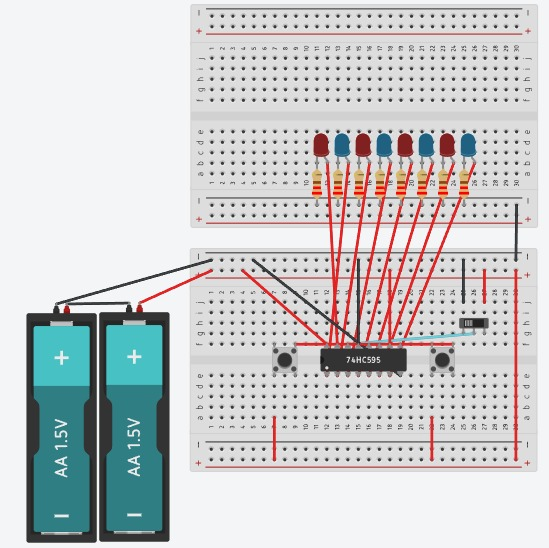
\includegraphics[width=7cm]{74HC595.jpg}
\centering
\caption{Circuito independiente 74HC595.}
\label{fig:74HC595.jpg}
\end{figure}



\subsection{Comunicación entre Arduinos}
Para realizar la comunicación entre arduinos realizamos dos señales en el arduino transmisor (Arduino 1), las cuales son la señal de datos y la del reloj. \\

Para las señales de datos se utilizaron varias señales de prueba. Las señales de prueba para los datos fueron las siguientes:
\begin{itemize}
\item 01110010
\item 00110101
\item 10001100
\item 11111101010100101
\end{itemize}

La lectura de los datos se hará con cada flanco de subida del reloj.\\

Las señales de prueba se realizaron en el loop de Arduino y se utilizaron funciones delay. Los tiempos de delay se utilizan para entender cuándo se deben hacer modificaciones tanto en las señales de datos como en las del reloj.\\

Por ejemplo; para la primera señal de prueba para los datos, las señales de datos y de reloj se pueden observar como las señales de la figura 2, en donde t2 corresponde al tiempo entre la generación del bit de la señal de dato y el flanco de subida del reloj, y t1 corresponde al periodo de la señal de reloj.\\

\begin{figure}[h]
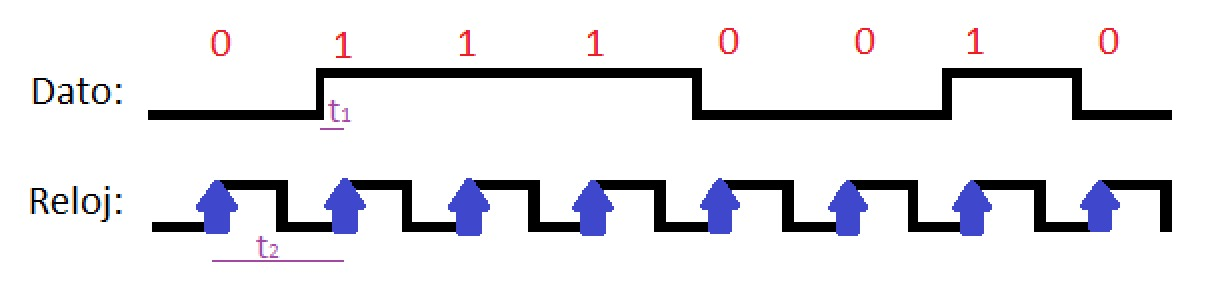
\includegraphics[width=12cm]{Prueba_datos_y_clock.jpeg}
\centering
\caption{Señales para la primera prueba de la señal de dato}
\label{fig:Prueba_datos_y_clock.jpeg}
\end{figure}

Para el t2 de la prueba, su valor es de 1 segundo. Se utilizan 500 milisegundos para el valor en alta y 500 milisegundos en baja. Para t1 se utiliza un valor de 250 milisegundos.\\


Para la interconexión entre los arduinos se realiza el monje de la figura 3, en donde en el arduino 1 el puerto 6 es la señal del reloj, el puerto 7 es la del bit a recolectar, y el puerto 6 del arduino 2 es el bit que se recibió visto como flanco.
\newpage


\begin{figure}[h]
\includegraphics[width=7cm]{interconexión del arduino.PNG}
\centering
\caption{Interconexión de los Arduinos}
\label{fig:interconexión del arduino.PNG}
\end{figure}

Basados en la figura 2, se realizan los códigos en Arduino.\\


Las figuras 4, 5 y 6 muestran el código en el arduino de transmisión.\\

\newpage

\begin{figure}[h]
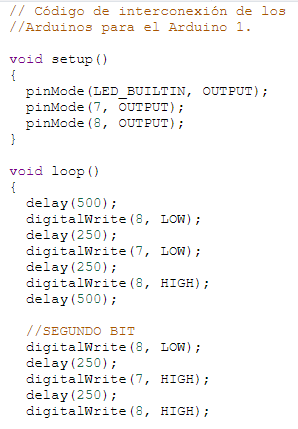
\includegraphics[width=8cm]{codigo_arduino1_1.PNG}
\centering
\caption{Primera parte del código del Arduino transmisor.}
\label{fig:codigo_arduino1_1.PNG}
\end{figure}

\newpage

\begin{figure}[h]
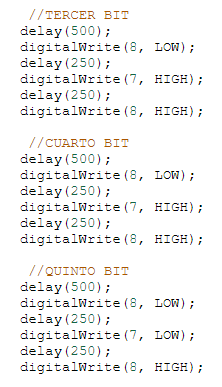
\includegraphics[width=5cm]{codigo_arduino1_2.PNG}
\centering
\caption{Segunda parte del código del Arduino transmisor.}
\label{fig:codigo_arduino1_2.PNG}
\end{figure}

\newpage

\begin{figure}[h]
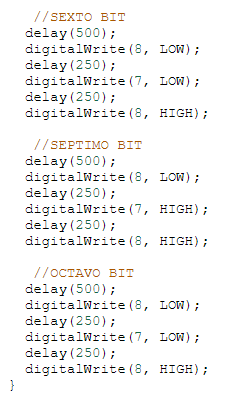
\includegraphics[width=5cm]{codigo_arduino1_3.PNG}
\centering
\caption{Tercera parte del código del Arduino transmisor.}
\label{fig:codigo_arduino1_3.PNG}
\end{figure}


La figura 7 muestra el código en el arduino de recepción.\\

\newpage


\begin{figure}[h]
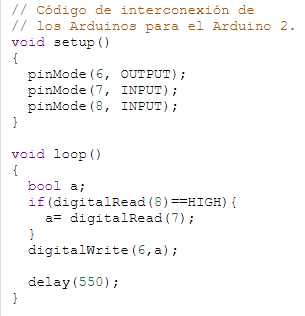
\includegraphics[width=7cm]{codigo_arduino2.PNG}
\centering
\caption{código del Arduino receptor.}
\label{fig:codigo_arduino2.PNG}
\end{figure}

\newpage
\subsection{Sistema de desencriptación.}

Para el sistema de desencriptación se utiliza un circuito integrado 74HC04 y dos 74HC08, los cuales corresponden a un circuito integrado de compuertas inversoras y de compuertas AND respectivamente.

Se usan 3 compuertas inversoras y 7 compuertas AND, siguiendo el esquema de la figura XXXXX. Se utilizaron compuertas AND debido a que estas son compuertas que sólo obtienen un '1' para un caso, por lo que para otros casos en que no sean el solicitado arrojan '0'.


\begin{figure}[h]
\includegraphics[width=7cm]{compuertas_sistema_desencriptación.PNG}
\centering
\caption{}
\label{fig:compuertas_sistema_desencriptación.PNG}
\end{figure}



El esquema de arduino para la implementación del esquema de la figura anterior junto con las compuertas lógicas es el de la figura XXXXX, y el código que se implementó para observar el buen funcionamiento del circuito es el de la figura XXXX, en el cual se mandan los bits correspondientes a la clave individual del grupo, el número 171, el cual en bits corresponde al 10101011.


\begin{figure}[h]
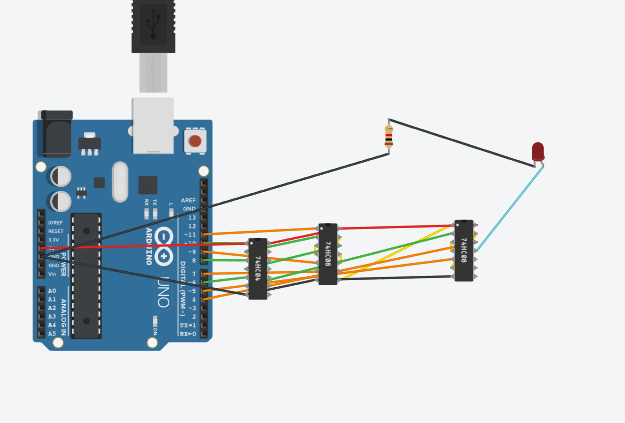
\includegraphics[width=7cm]{sistema_desencriptacion.PNG}
\centering
\caption{Sistema de desencriptación mediante compuertas lógicas.}
\label{fig:sistema_desencriptacion.PNG}
\end{figure}

\begin{figure}[h]
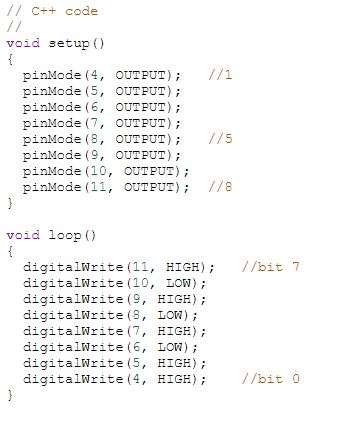
\includegraphics[width=8cm]{Desencrip1.JPG}
\centering
\caption{Código de prueba para la bandera del sistema de desencriptación.}
\label{fig:Desencrip1.PNG}
\end{figure}

\newpage



\subsection{Sistema completo}

\subsubsection{Arduino transmisor}

Para el arduino transmisor, se utilizaron 3 salidas, correspondientes a la señal de datos (pin 8), señal de reloj (pin 7) y una señal que se activa antes del noveno flanco de subida de la señal de reloj y se desactiva 0.1 segundos después (pin 6).\\


\begin{figure}[h]
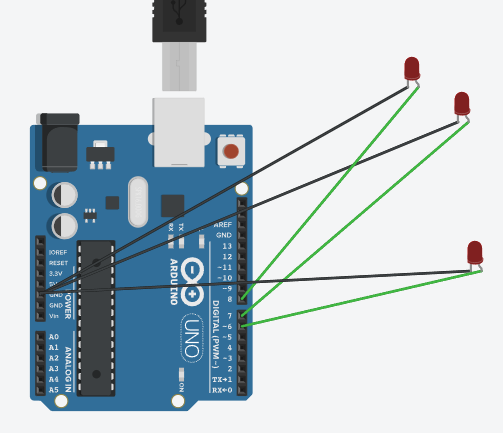
\includegraphics[width=7cm]{arduino_transmisor.PNG}
\centering
\caption{Circuito con Arduino configurado como transmisor.}
\label{fig:arduino_transmisor.PNG}
\end{figure}

La señal del pin 8 es la señal que entrega los datos en bits de los valores del arreglo entregado. La señal del pin 7 (señal de reloj) controla el almacenamiento de cada bit de la señal de datos, y la señal del pin 6 controla la señal que se ingresa al circuito integrado 74HC595 que da cuenta de cuándo se deben enviar los bits almacenados a la salida del integrado en forma paralela. La realización de estas señales se observa en el código para el circuito de transmisión en las figuras XXXXXX y XXXX. Se tiene en cuenta que la señal de datos debe tomar el valor deseado antes del flanco de subida del reloj, para esta se almacene adecuadamente, y que la señal del pin 6 debe generarse antes del noveno flanco de subida de la señal del reloj, para mostrar la cadena de 8 bits antes de recoger el noveno dato.\\


\begin{figure}[h]
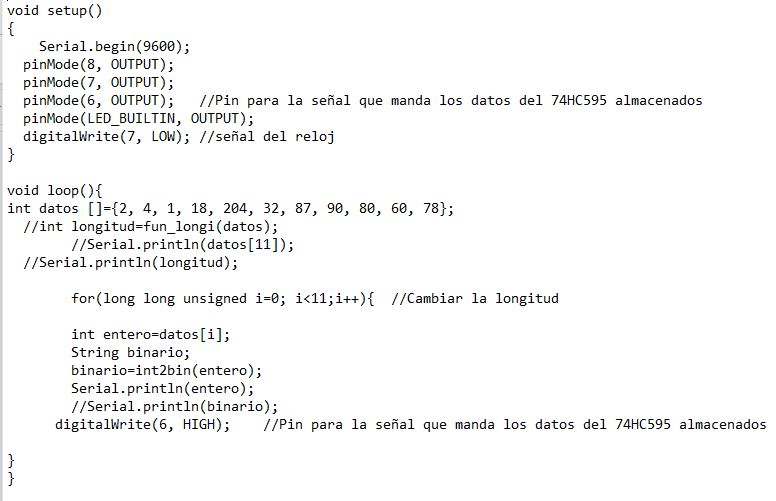
\includegraphics[width=11cm]{Transmisor1.JPG}
\centering
\caption{}
\label{fig:codigo_transmisor_1.PNG}
\end{figure}


\begin{figure}[h]
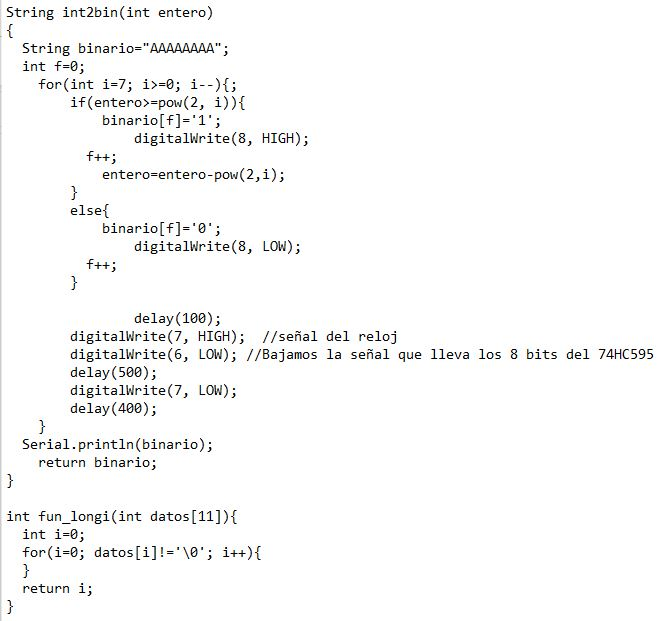
\includegraphics[width=11cm]{Transmisor2.JPG}
\centering
\caption{}
\label{fig:codigo_transmisor_2.PNG}
\end{figure}

Los datos importantes del código del arduito transmisor son la función int2bin (figura XXXX), la cual recoge el entero y lo transforma en string por medio de un for, el cual evalúa si su valor es mayor o igual a 2 a la séptima potencia, de ser así, se obtendrá un bit '1' en el bit más significativo. Así mismo se realizan con los demás bits. Además, en esta misma función se mandará por medio del puerto 8 el bit correspondiente a '1' o a '0' según es el caso. Al final de cada iteración del for, por tanto de cada envío de señal del dato en el puerto 8, se hace un delay de 0.1 segundos para generar la señal de subida del reloj. Además, al salir de la función (figura XXXX) se realiza el envío de la señal del puerto 6, para dar cuenta de que ya se cumplieron los envíos de los 8 bits.\\

Por medio de las 3 señales antes mensionadas y de la forma antes explicada se realiza una toma adecuada de los datos para el funcionamiento adecuado del circuito integrado 74HC595 y del arduino receptor.\\

\subsubsection{Arduino transmisor y Circuito 74HC595}

\begin{figure}[h]
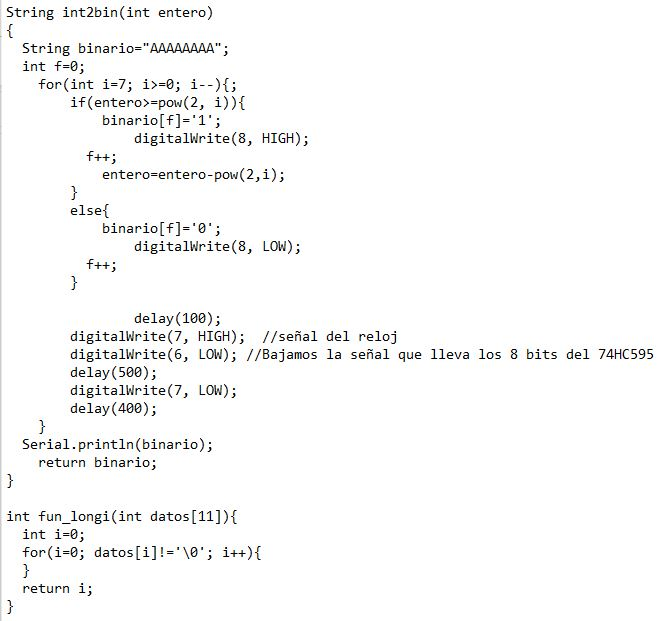
\includegraphics[width=11cm]{Transmisor2.JPG}
\centering
\caption{}
\label{fig:conexion_arduino_con_74HC595.PNG}
\end{figure}

En la interconexión del arduino con el circuito integrado 74HC595, se interconectar el pin 8, 7 y 6 del arduino con los pines 14, 11 y 12 del 74HC595 respectivamente.

Se agregan LEDs para observar la serie de bits que arroja el integrado. Estos bits están ordenados por orden de peso de bit.

\subsubsection{Arduino transmisor y Circuito 74HC595}

Para realizar el circuito de desencriptación, se sigue el esquema de la figura XXXXXXX. Este esquema cambió respecto al numeral 1 en que se modifica un circuito de 4 AND de 2 entradas por un circuito de 2 AND de 4 entradas.


\section{CONCLUSIONES} \label{conclulsion}
\begin{itemize}
\item La plataforma de Tinkercad, el microcontrolador Arduino, el lenguaje C++ y el circuito integrado 74HC575 son piezas claves tanto para la realización de este proyecto como para la realización de otros proyectos prácticos.
\item El microcontrolador Arduino es útil para el envío de información a otras plataformas para otros lenguajes de programación, y también a otros arduinos.
\item El uso del circuito integrado es útil para el envío paralelo de los datos.

\end{itemize}

\section{REFERENCIAS}    

\bibliographystyle{IEEEtran}

\bibliography{references}

\end{document}
